\ifx\wholebook\relax \else

\documentclass[b5paper]{article}
\usepackage[nomarginpar
  %, margin=.5in
]{geometry}

\addtolength{\oddsidemargin}{-0.05in}
\addtolength{\evensidemargin}{-0.05in}
\addtolength{\textwidth}{0.1in}

\usepackage[en]{../prelude}

\setcounter{page}{1}

\begin{document}

\title{Numerals}

\author{Xinyu LIU
\thanks{{\bfseries Xinyu LIU} \newline
  Email: liuxinyu99@hotmail.com \newline}
  }

\maketitle
\fi

\markboth{Numerals}{A tour of numbers}

\ifx\wholebook\relax
\chapter{Numerals}
\fi

\epigraph{The total number of minds in the universe is one.}{Erwin Schrödinger}

Numbers appear everywhere in our daily life. Here's a piece of news pops up: \textit{The 2024 Paris Olympic Games to an end on Sunday August 11, 2024. Paris is the second city, after London, to host the Summer Olympics three times. It set a record of gender equality, with 5,250 male and 5250 female athletes. In total, 32 sports and 329 events were featured, with 206 countries and regions participating. Four new sports made their debut: skateboarding, surfing, sport climbing, and breakdancing. A total of 329 gold medals were up for grabs. Athletes from various countries and regions demonstrated outstanding athleticism. The United States and China tied for the most gold medals, with each securing 40. The United States also led in silver medals with 44 and bronze medals with 42.} There are 14 numbers among the 120 words in this news. We don't know who invented the numerals because they show up with text in almost all history documents to the very early time. Some believe numerals arose with language. Anthropologists identified numbers inscribed in bones, stones, caves, clay, etc. We can also find such clues in our languages, for example in English, eleven comes from `endleofan', meaning (ten) left one; twelve comes from `twelf', meaning left two.

\section{Rosetta stone}
\index{Rosetta stone}

\begin{figure}[htbp]
 \centering
 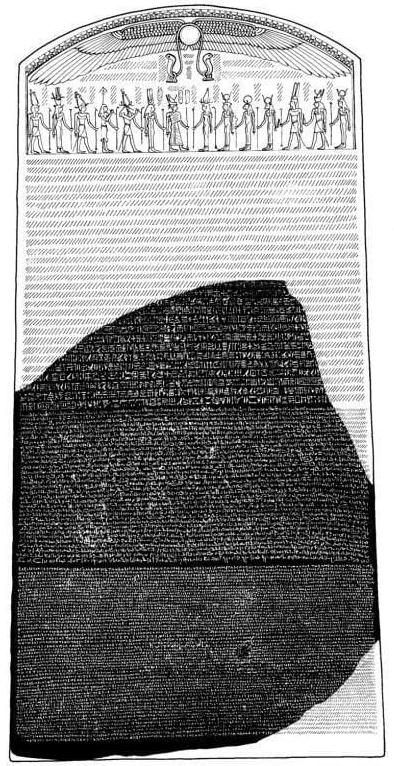
\includegraphics[scale=0.5]{img/Rosetta-stone-recons}
 \caption{Rosetta stone was broken in the middle.}
 \label{fig:rosetta-stone-recons}
\end{figure}

There is a famous stone in room 4, the British museum.

\ifx\wholebook\relax \else
\section{Answer}
\shipoutAnswer

\begin{thebibliography}{99}

%% \bibitem{wiki-number}
%% Wikipedia. ``History of ancient numeral systems''. \url{https://en.wikipedia.org/wiki/History_of_ancient_numeral_systems}

%% \bibitem{Calvin-Clawson-1994}
%% Calvin C Clawson. ``The Mathematical Traveler, Exploring the Grand History of Numbers''. Springer. 1994, ISBN: 9780306446450

%% \bibitem{wiki-babylonian-num}
%% Wikipedia. ``Babylonian numerals''. \url{https://en.wikipedia.org/wiki/Babylonian_numerals}

\end{thebibliography}

\expandafter\enddocument
%\end{document}

\fi
